\newpage
\appendix

\section{Visualization of cleaned vs raw dataset}

\begin{figure}[!h]
    \centering
    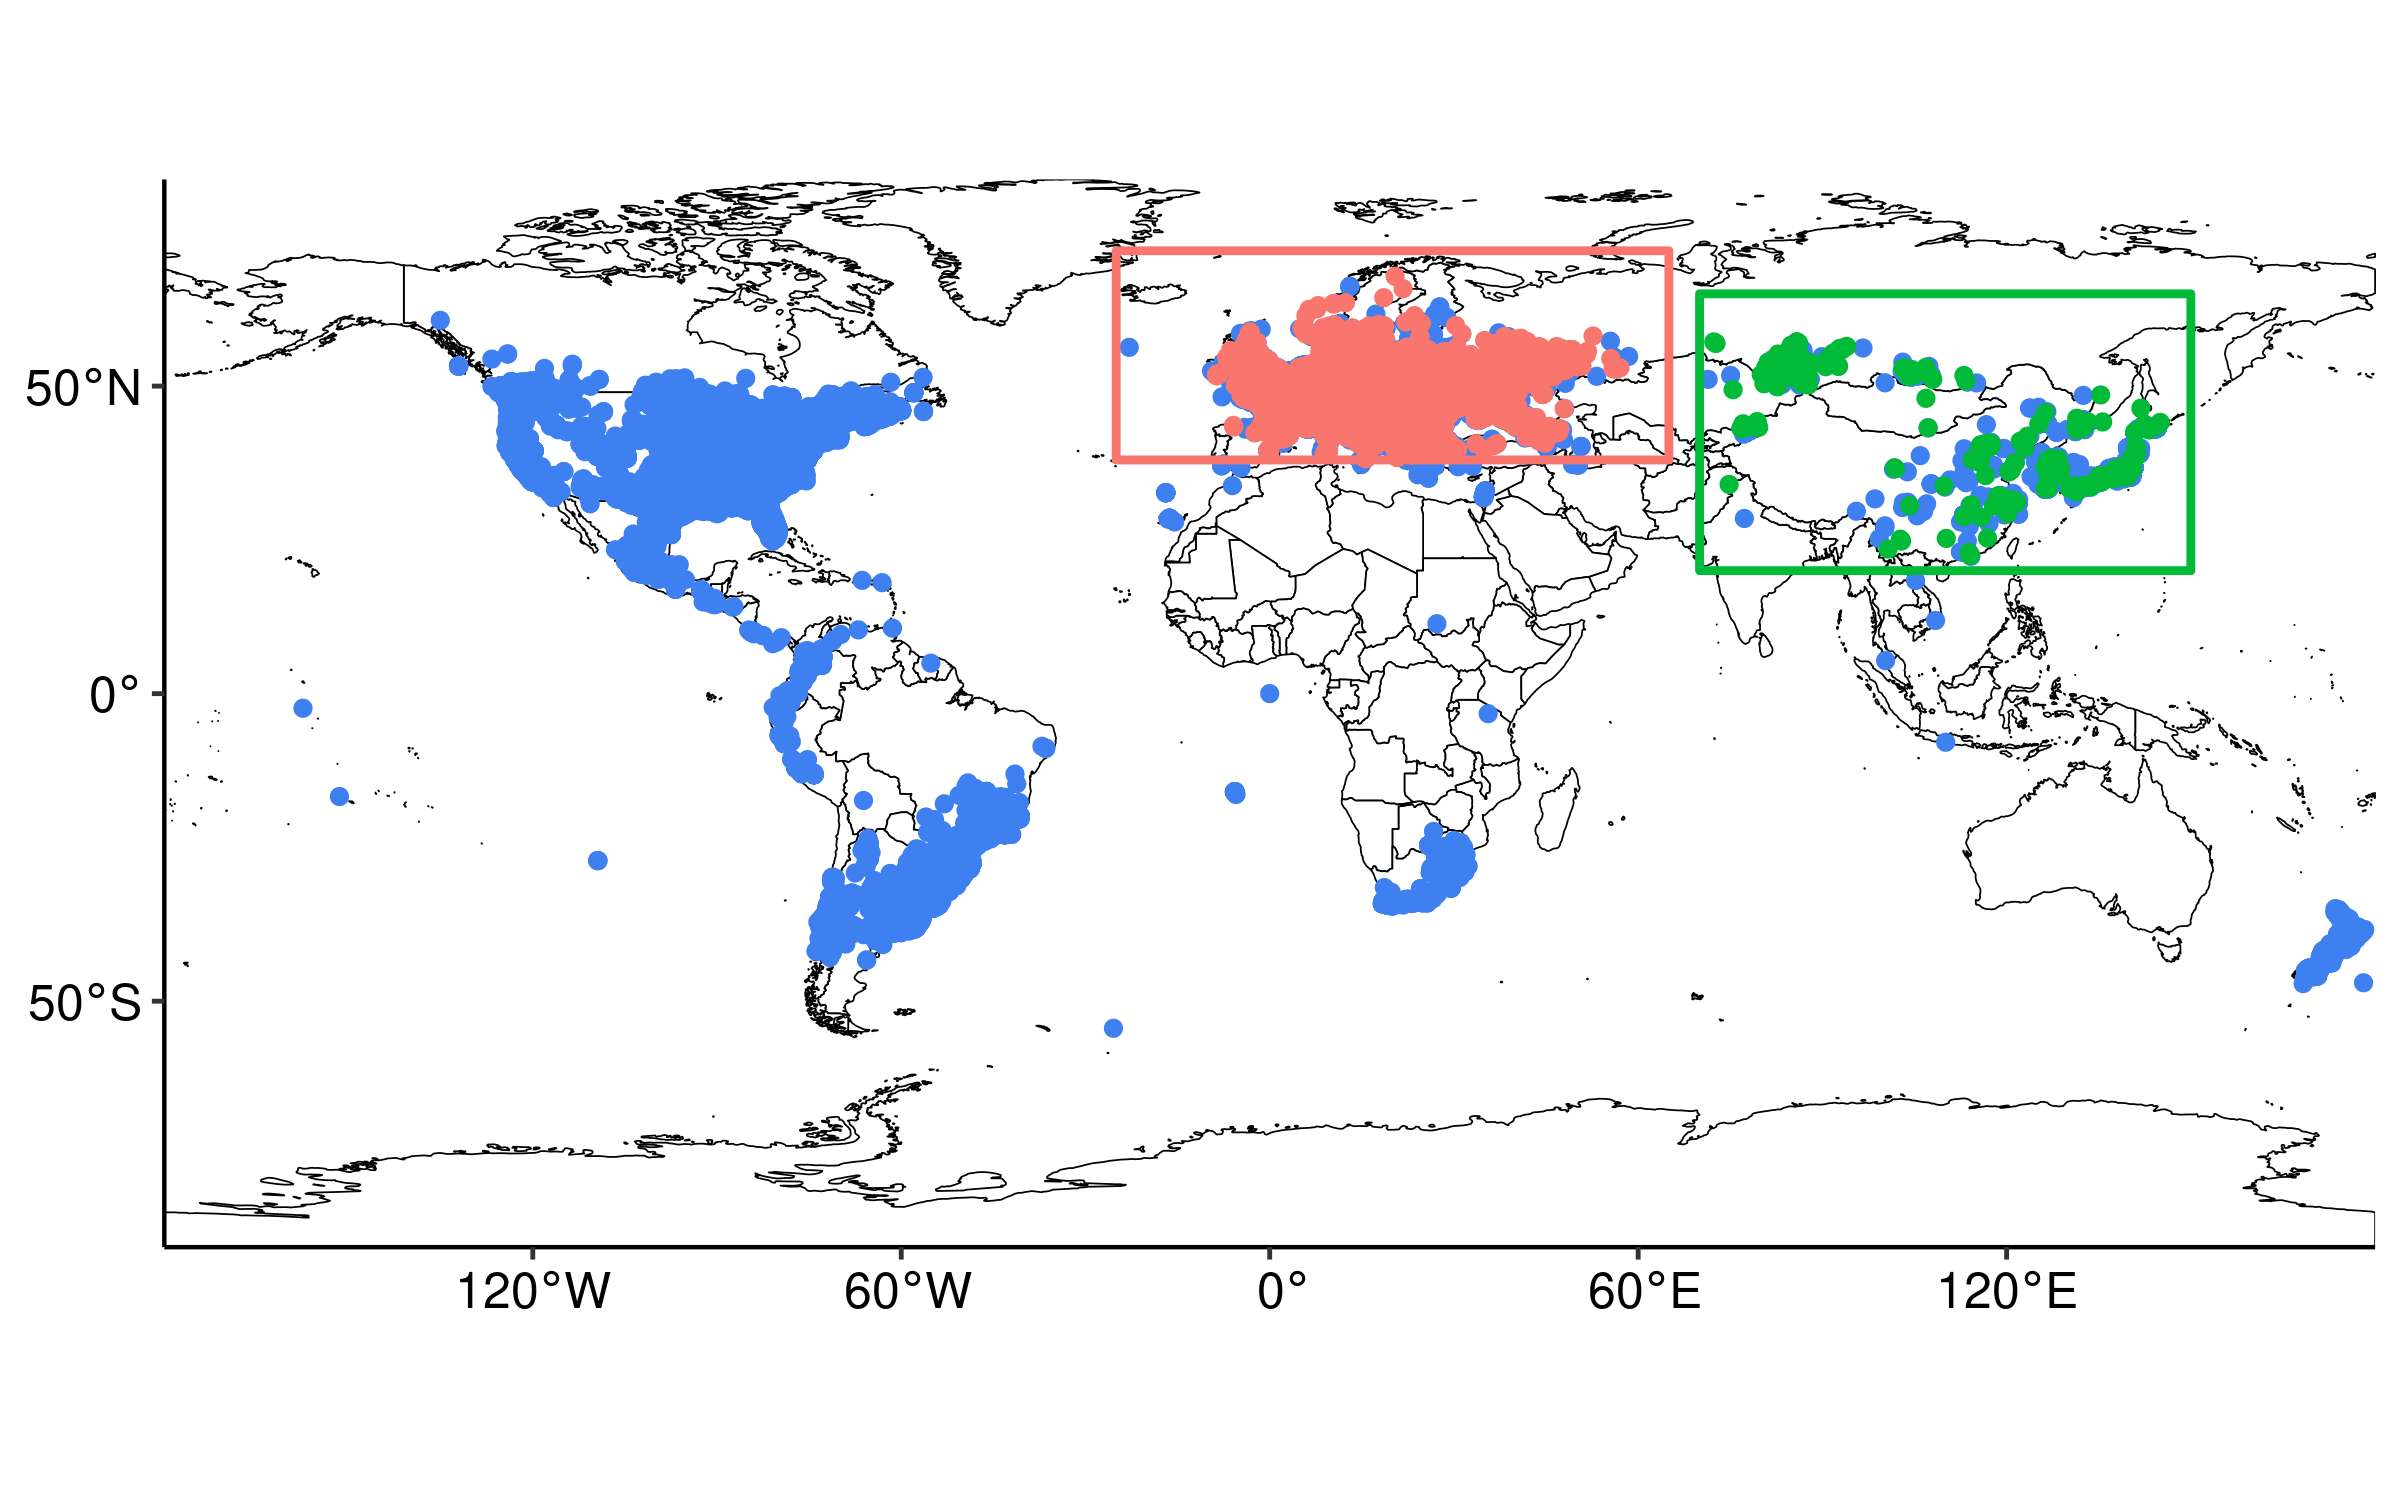
\includegraphics[width = 0.9\linewidth]{"../../R/figures/raw-vs-cleaned-glob.png"}
    \caption{\label{fig:raw_vs_cleaned_glob} Visualization of the cleaned dataset for \gls{harm} in comparison to the total raw dataset. The red and green boxes show the used extents for Europe and the native range respectively, red and green points show the cleaned presence points in their respective extents, while blue points show all points of the raw dataset.}
\end{figure}

\section{Niche analysis for native and invaded niche}

\begin{figure}[!h]
    \centering
    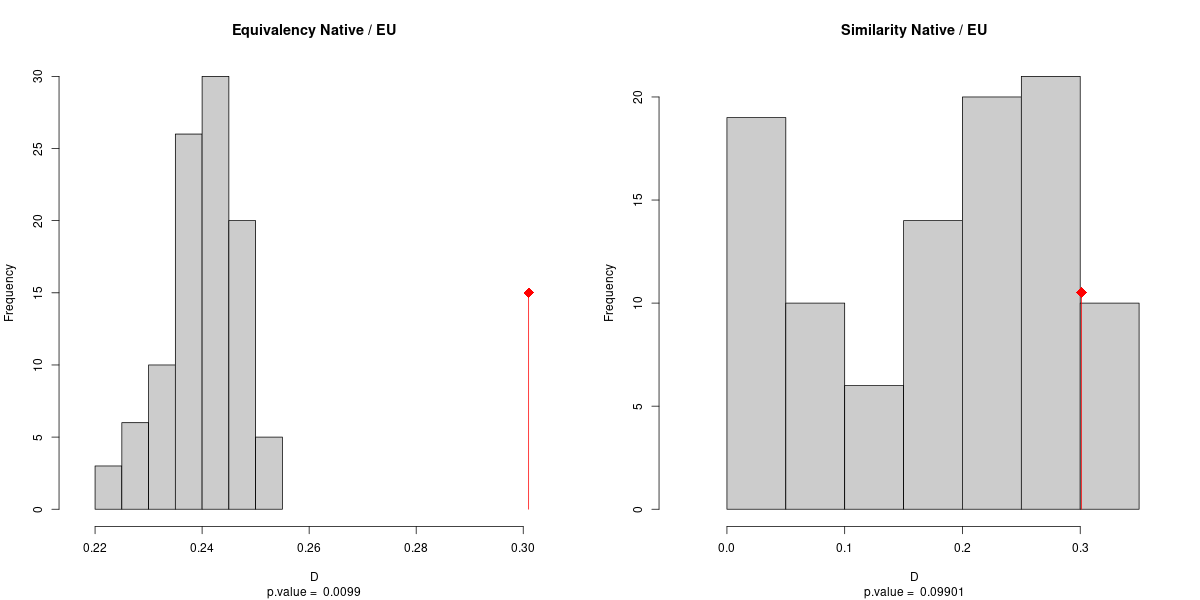
\includegraphics[width = \linewidth]{"../../R/figures/as-eu-tot-eq-sim.png"}
    \caption{\label{fig:as_eu_eq_sim} Results of the niche equivalency (left) and niche similarity (right) test comparing the native and invaded niche of \gls{harm}. Histograms of the simulated niche overlaps, the observed overlap shown as a red bar with a diamond.}
\end{figure}

\begin{figure}[!h]
    \centering
    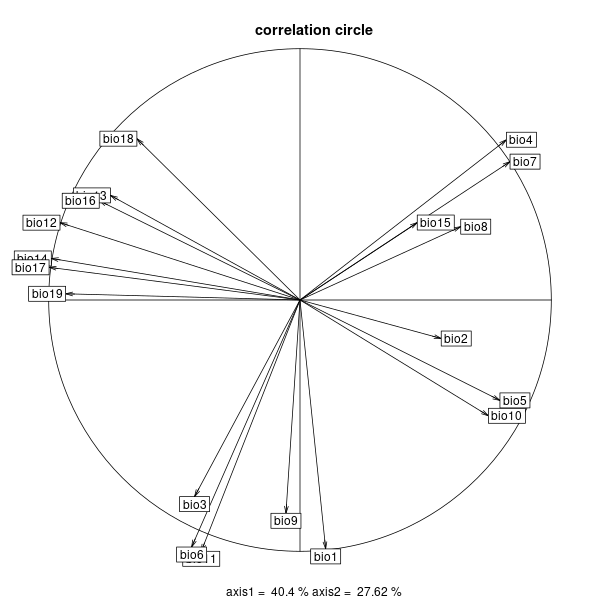
\includegraphics[width = 0.7\linewidth]{"../../R/figures/as-eu-pca.png"}
    \caption{\label{fig:as_eu_niche_pca} Component contributions for the PCA used to conduct the niche analyses comparing the total native and invaded niches. For detail on the bioclim variables, see (Supplementary Table \ref{tab:bioclim})}
\end{figure}

\begin{figure}[!h]
    \centering
    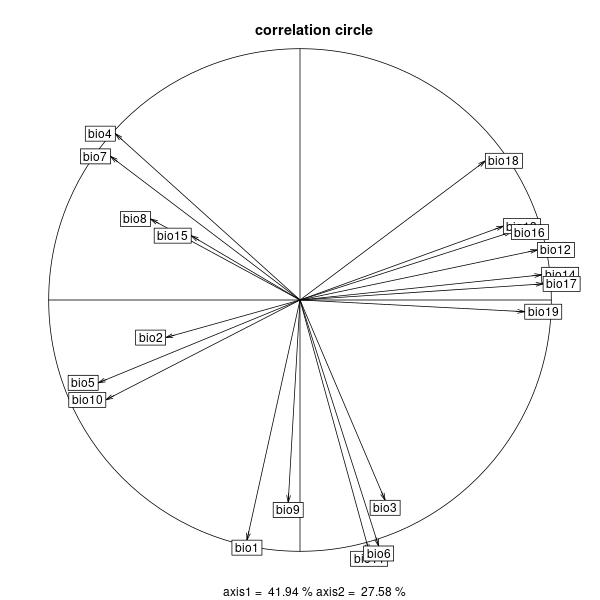
\includegraphics[width = 0.7\linewidth]{"../../R/figures/eu-years-pca.png"}
    \caption{\label{fig:eu_years_pca} Component contributions for the PCA used to conduct the niche analyses comparing each year of the invaded niche to its  following year. For detail on the bioclim variables, see (Supplementary Table \ref{tab:bioclim})}
\end{figure}

\begin{table}[!h]
    \centering
    \caption{\label{tab:bioclim} Explanation of the bioclim variables (from CHELSA 2.x technical specifications).}
    \begin{tabular}{l l}
        \textbf{variable} & \textbf{explanation}
        \csvreader[head to column names]{tab-CHELSA-bioclim-expl.csv}{}{
        \\ \shortname & \longname
        }
    \end{tabular}
\end{table}

\section{Species distribution models}